\subsection{Experimental Analysis}
%
To confirm the theoretical results obtained in section \ref{subsec:intro}, two experimental setups will be created. In the first experiement, we will study quantum noise in the single homodyne detection. The experimental setup will be based on the paper \cite{chi2011balanced}. In the second experiment, we will study quantum noise in the double homodyne detection setup, which will be basically an extension of the single homodyne detection setup.\\
\\
\subsubsection{Single homodyne detection}
%
To keep the experiment simple and avoid extra sources of noise, we will avoid using black boxes wich have complicated inner workings, having a preference in using simple components, as shown in fig. \ref{fig:experimental_homodyne_setup}:
\\
\begin{figure}[H]
	\centering
	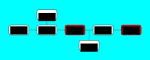
\includegraphics{./sdf/optical_detection/figures/scheme_experimental.pdf}
	\caption{Experimental setup}
	\label{fig:experimental_homodyne_setup}
\end{figure}
%
%
Material list
\begin{table}[H]
	\centering
	\begin{tabulary}{1.0\textwidth}{|L|L|l|}
		\hline
		\textbf{Device}		& \textbf{Description}\\
		\hline
		Local Oscillator	& Yenista OSICS Band C/AG\\
		\hline
		BS					& Beam Splitter\\
		\hline
		Pulse Generator		& HP 8116A Pulse Generator\\
		\hline
		Amplitude Modulator	& Mach Zehnder SDL OC 48\\
		\hline
		VOA					& Eigenlicht Power Meter 420\\
		\hline
		VOA					& Thorlabs VOA 45-APC\\
		\hline
		PIN					& Thorlabs PDB 450C\\
		\hline
		ADC					& Picoscope 6403D\\
		\hline
	\end{tabulary}
\end{table}
%
A single laser is splitted and used as the source for the signal (S) and the local oscillator (LO). The signal beam is pulsed and highly attenuated. The local oscillator is also attenuaded, but not pulsed. The signal and local oscillator interfere in a Beam Splitter originating two beams which are then converted to voltages in the PIN. These voltages are read in the Digital Oscilator (OSC) and collect in the computer. In the post processing phase, the quantum noise is measured by applying a difference between the two beams and measuring it's variance.
\\
The second stage of the experiment will be very similar to the first one, in which the signal and local oscillator branches will be divided. One of the new branches of the local oscilator will suffer a phase delay of $\pi/2$, in order to measure the quadrature component of the incoming signal.\\
%%
%%
\subsubsection{Thorlabs detector}
%%
The detector used in the laboratory is the Thorlabs PDB 450C. This detector consists of two well-matched photodiodes and a transimpedance amplifier that generates an output voltage (RF OUTPUT) proportional to the difference between the photocurrents of the photodiodes.\\
Additionally, the unit has two monitor outputs(MONITOR+ and MONITOR-) to observe the optical input power level on each photodiode separately.
\cite{pdb450Cmanual}
%
\begin{figure}[H]
	\centering
	\includegraphics{./sdf/optical_detection/figures/thorlabs-circuit.pdf}
	\caption{Thorlabs PDB 450 detection circuit.}
\end{figure}
%
%
The transimpedance amplifier (TIA) is an opamp-based current to voltage conversion amplifier.
\footnote{http://www.cypress.com/file/131966/download}
It is used in this circuit, given that the photodiode's current has a linear response to incident light in contrast to it's non-linear voltage response.
\footnote{http://www.ti.com/lit/an/sboa035/sboa035.pdf, p.1}
\\

We have seen that the theoretical results obtained in section \ref{sec:schemes} all depend on various parameters, such as amplitude, bandwidth, amplification, frequency response and noise.
Therefore, we need to characterize our photodetector in order that our experimental results can show that our theoretical results are indeed correct.
%
%%
%%
%%++ ITEMS DO PROF ++\\
%- responsividade do pin1 e do pin2
%- ganho do meu amplificar OPAMP
%- largura de banda
%- formado filtro, espectro do filtro
%- ruído térmico, no braço superior, no braço intermédio e no braço inferior
%%
%%
\\
Table \ref{table:thorlabs} lists various important characteristics to perform our measurements. These values were obtained from the device's manual \cite{pdb450Cmanual}
\begin{table}[H]
	\centering
	\begin{tabulary}{1.0\textwidth}{|L|L|l|}
		\hline
		\textbf{Characteristic}			& \textbf{Value}\\
		\hline
		Bandwidth (monitor)				& DC to 1 MHz\\
		\hline
		Voltage Gain (monitor)			& 10 V/mW @ peak responsivity\\
		\hline
		Voltage Noise (monitor)			& <180 \textmu V (RMS)\\
		\hline
		Max Responsivity (PIN)			& 1.0 A/W\\
		\hline
		RF OUTPUT Bandwidth(-3dB)		& DC to 150 / 45 / 4 / 0.3 / 0.1 MHz\\
		\hline
		RF OUTPUT Transimpedance Gain	& $10^3$ / $10^4$ / $10^5$ / $10^6$ / $10^7$ V/A\\
		\hline
		RF OUTPUT Conversion Gain		& $10^3$ / $10^4$ / $10^5$ / $10^6$ / $10^7$ V/W\\
		\hline
	\end{tabulary}
	\caption{Main characteristics of the Thorlabs PDB450C balanced detector}
	\label{table:thorlabs}
\end{table}
%%
%%
\noindent
{\bf Gain response}\\
The gain response is obtained by fixing an frequency $\omega_0$ and generating optical signals with various amplitudes $A_i$, such as $V = A_i \sin \left( \omega_0 t \right)$ and reading the output voltage amplitude.
\footnote{REF?}\\
\\
{\bf Frequency response/Bandwidth}\\
The frequency response is obtained by fixing an amplitude $A_0$ and generating  optical signals with various frequencies $\omega_i$, such as $V = A_0 \sin \left( \omega_i t \right)$ and reading the output voltage amplitude.
\footnote{REF?}
\\
The following plot shows the gain for various frequencies???
\begin{figure}[H]
	\centering
	\includegraphics[width=10cm]{./sdf/optical_detection/figures/thorlabs-manual-gain-spec-rf.png}
	\caption{Thorlabs PDB 450 RF output amplitude with frequency, for various gain values.\\(Plots from the manual)}
\end{figure}
%%
%%
\subsubsection{Data analysis}
%
Using the data collected in the Digital Oscilloscope, we process each sample for each power level (which???).
This data analysis will consist in the following steps:
1) Subtract the data coming from MONITOR- from the data from MONITOR+.\\
2) Calculate the average impulse and the variance of the impulse. (VALE A PENA ESPECIFICAR A EQUIVALÊNCIA DE FASE?)\\
3) The representative variance will be the variance of the pulse maximum.\\\
%
For each combination of the expected number of photons present in the signal and the local oscillator, we will obtain the variance in the plateau of the pulse. The final variance is simply the mean of the variances of all pulses.
%

\subsubsection{Double homodyne detection}
%
%-- UNDER CONSTRUCTION --\\
The experiemental setup for this experiment is a simple extension of the single homodyne detection. To implement this experiment, the signal beam will be divided in two beams, in which one of them will be detect in phase with local oscillator and the other in phase with a an oscillator with a $pi/2$ phase relative to the first one.
%

\subsection{Comparative analysis}
%
%WARNING -- OLD DATA --\\
%
Given the theoretical, simulated and experimental frameworks, we will now compare the results obtained by each of them.
\\
%
\begin{figure}[H]
	\begin{subfigure}{.5\textwidth}
		\centering
		\includegraphics[width=.8\linewidth]{./sdf/optical_detection/figures/noise_exp_channel1.png}
		\caption{$X$ quadrature}
		\label{fig:noise-exp-1}
	\end{subfigure}%
	\begin{subfigure}{.5\textwidth}
		\centering
		\includegraphics[width=.8\linewidth]{./sdf/optical_detection/figures/noise_exp_channel3.png}
		\caption{$Y$ quadrature}
		\label{fig:noise-exp-3}
	\end{subfigure}
	\captionsetup{justification=centering}
	\caption{Noise variance dependency with local oscilator power for two different quadratures. Experimental vs fitted data.}
\end{figure}
%
Figures $\ref{fig:noise-exp-1}$ and $\ref{fig:noise-exp-3}$ show measurements of total noise for two different quadratures. For low power of LO, the noise variance flutuates around a constant value. For high power of LO, $(P_{LO}>10^{-4}W)$, the variance of noise shows an increasing trend roughly proportional to $P_{LO}^2$. The polynomial fittings confirm this trend, showing a degree 2 coefficient much larger than the degree 1 coefficient
%
\begin{equation}
\textrm{Var}_X = 2.22 \!\! \times \!\! 10^{-5} + 9.6 \!\! \times \!\! 10^{-3} P_{LO} + 3.40 P_{LO}^2
\end{equation}
\begin{equation}
\textrm{Var}_Y = 2.71 \!\! \times \!\! 10^{-5} + 8.9 \!\! \times \!\! 10^{-3} P_{LO} + 7.25 P_{LO}^2
\end{equation}
%
The expected growth should be proportional to $P_{LO}$, but the RIN noise, originated by the electric apparatus, which grows quadratically with the power, is dominating the noise amplitude for large $P_{LO}$.\\
We see that both the simulation and experimental data display a similar behaviour, but the quadratic growth of noise for large $P_{LO}$ was not predicted in the simulations.\\ 